\subsection{Word segmentation}
\label{sec:segmentation}


Does the model develop an implicit notion of word?

English/German/Italian

How validation partition was used

Use only one of the low-parameter-count methods, compare to Bayes
although it's not entirely fair (clarify that). (report in text or
footnote that, when training on the hidden state, we get super-high
accuracy, indicating that the information is there).

LSTM vs RNN vs Bayes vs n-gram baseline (collect transition
probabilities across fixed n-gram windows, optimize threshold on
validation data).

Results could be summarized as in Table \ref{tab:segmentation-results}.

How reliable is this signal?


We constructed a logistic classifier taking into account (1) log-probability of the next character, (2) entropy of the distribution over the next character, (3) the total likelihood of the next 25 characters, minus the unconditional likelihood estimated by starting the CNLM at the current position.
The rationale of (3) is that it measures the pointwise mutual information, and thus the statistical association, between the subsequent characters and the prior context.
It is also the transition probability for the next characters
We collected these quantities for each position and for the preceding and following three characters.
In total, the classifier has 21 coefficients.

We also conducted the same experiment with a character-level 8-gram model estimated on the training set.

The goal of this experiment is not to construct a word segmentation system, but to evaluate how strongly the CNLM's probabilities are indicative of word boundaries.


\begin{table}[t]
  \begin{center}
    \begin{tabular}{l|l|l|l|l}
      \multicolumn{1}{c}{}&\emph{LSTM}&\emph{RNN}&\emph{8-grams}\\
      \hline
      English & 65.83/60.37/62.98 &   63.26/59.81/61.49 & 55.73/51.0/53.26    \\ % \ldots{}/\ldots{}/\ldots & \ldots{}/\ldots{}/\ldots & \ldots{}/\ldots{}/\ldots &\ldots{}/\ldots{}/\ldots\\
      German &  57.012/52.505/54.67 &  53.2/49.26/51.15 & 42.89/36.28/39.31   \\ %   \ldots{}/\ldots{}/\ldots & \ldots{}/\ldots{}/\ldots & \ldots{}/\ldots{}/\ldots &\ldots{}/\ldots{}/\ldots\\
      Italian &  63.59/56.95/60.09 & 62.47/57.5/59.89  & 48.41/39.62/43.57    \\ % \ldots{}/\ldots{}/\ldots & \ldots{}/\ldots{}/\ldots & \ldots{}/\ldots{}/\ldots &\ldots{}/\ldots{}/\ldots\\
    \end{tabular}
  \end{center}
  \caption{\label{tab:segmentation-results} Precisionm recall, and F1 on word segmentation.}
\end{table}

Results are shown in Figure~\ref{tab:segmentation-results}.
%PMI alone 
%P 30.56 R 20.61 F 24.61 German
%P 32.19 R 20.89 F 25.34 Italian
%P 39.37 R 29.45 F 33.69 English
%Surprisal alone
%P 28.04 R 18.64 F 22.4 German
%P 28.76 R 18.31 F 22.38 Italian
%P 33.65 R 24.1 F 28.08 English
%Entropy alone
%P 50.88 R 45.57 F 48.08 German
%P 58.44 R 52.09 F 55.08 Italian
%P 59.85 R 53.75 F 56.63 English


Ablation shows that the entropy is most predictive, reaching an F1 of 56.63 (English), 48.08 (German), 55.08 (Italian) alone.
Surprisal reaches 28.08 (English), 22.4 (German), 22.38 (Italian); PMI reaches 33.69 (English), 24.61 (German), 25.34 (Italian).
%Setting N to other values shows that larger values of N increase performance (N =10: 62.45, N=20: 63.24).

\begin{figure}
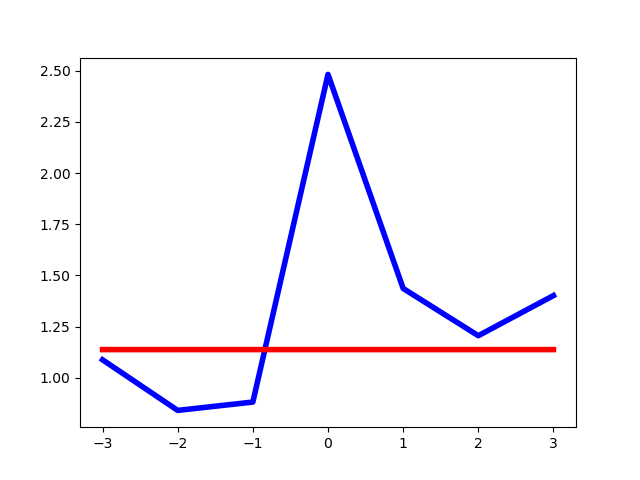
\includegraphics[width=0.22\textwidth]{figures/segmentation-profile-flattened-entropies-german.png}
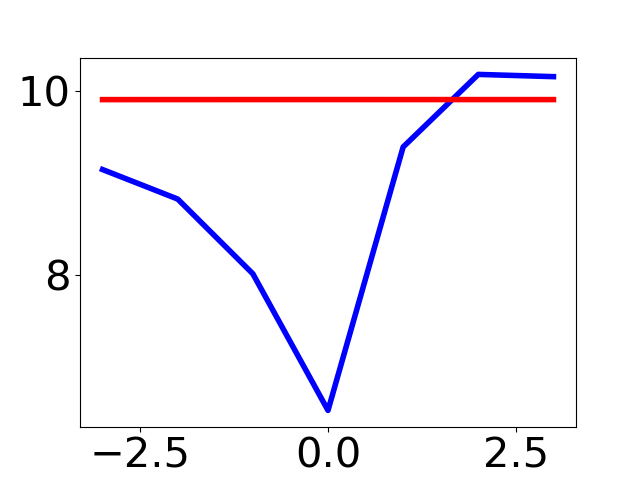
\includegraphics[width=0.22\textwidth]{figures/segmentation-profile-flattened-pmis-german.png}
	\caption{Entropy and PMI at word boundaries (blue), compared to all positions (red). }\label{fig:syntax-depth}
\end{figure}

How does the LSTM CNLM compare to unsupervised word segmentation models?
Running Bayesian methods on the Wikipedia dumps is infeasible; thus we also created a CNLM on the Brent corpus.

\begin{table}[t]
  \begin{center}
    \begin{tabular}{l|l|l|l|l}
      \multicolumn{1}{c}{}&P/R/F & Lexical & Boundaries\\      \hline
      CNLM & 0.75/0.76/ & 0.41/0.61 & 0.91/0.90 \\
     pmi & 0.708/0.729 \\
     entropy & 0.504/0.533 \\
     likelihood & 0.453/0.510 \\
      Goldwater 2006 & 0.740/0.794 & 0.679/0.589
    \end{tabular}
  \end{center}
  \caption{\label{tab:segmentation-results-brent} Word segmentation results on the Brent corpus.}
\end{table}

Results in Table~\ref{tab:segmentation-results-brent} show that the performance is broadly comparable to that of a sophisticated Bayesian segmentation method.
In contrast to the Wikipedia experiments, pmi emerges as the most important predictor on this dataset.

Unlike our method, the Bayesian method is fully unsupervised, but it has an .

Note that, unlike supervised word segmentation methods, our classifier does not have access to the character strings directly; instead, it evaluates how strongly quantities computed by the CNLM \emph{correlate} with word boundaries.



Looking at the main errors made by our English CNLM is instructive. We
consider first the 30 most common undersegmentations in the test set
(that is, cases in which the model failed to split two or more
words). About half (16) of them are common function word sequences
that could indeed easily be re-analyzed as single words (e.g.,
\emph{more than}, \emph{as well as}, \emph{such as}). Of the remaining
cases, 8 follow the \emph{N of} pattern, where \emph{N} is a
(typically relational) noun commonly occurring in this construction
(\emph{member of}, \emph{end of}, \emph{part of}\ldots). There are 3
fixed multi-word expressions (\emph{New York}, \emph{United States}
and \emph{high school}). Finally, it's reasonable to treat \emph{based
  on}, \emph{known as} and \emph{according to} as lexicalized
connectives, especially in the Wikipedia text the model was trained
upon.

The picture is a bit murkier but still fairly linguistically grounded
for the 30 most common oversegmentation errors (that is, the character
fragments that are wrongly segmented from inside the largest number of
distinct words).\footnote{We ignore here single-letter segmentations,
  that would otherwise account for one third of the most-frequent
  set.}  More than half (17) are common affixes (prefixes such as
\emph{re} and \emph{de} or suffixes such as \emph{ing} and
\emph{ly}). The remaining cases include 3 strings identical to frequent
function words wrongly carved out of longer words (\emph{the},
\emph{to} and \emph{on}, although the model might be treating the
latter as a pseudo-suffix in forms such as \emph{Peterson} and
\emph{Creighton}). Further, the strings \emph{land} and \emph{man} are not
unreasonably segmented out of compounds. It's hard, on the other hand,
to find a linguistically sound motivation for the 8 remaining top
oversegmentations (\emph{la, le, ma, na, ra, ro, se, ta}).


We hypothesized that the same might be true for hierarchical syntactic structure.
We created constituency trees for the German validation set using the Berkeley Parser~\ref{petrov2007improved}.
For each character in the data, we counted its hierarchical distance from the preceding character, operationalized as the number of intervening closing and opening brackets.
This number is zero if both characters belong to the same word.

Figure~\ref{fig:syntax-depth} plots MI by height.
The plot shows that longer hierarchical distance between neighboring characters corresponds to lower average MI.
This illustrates how it is useful for segmentation knowledge to be implicit, as the model ``knows'' about different kinds of boundaries in a continuous manner.

\begin{figure}
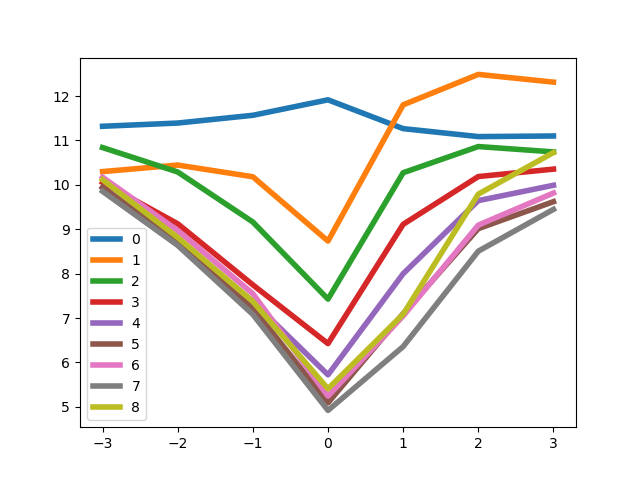
\includegraphics[width=0.48\textwidth]{figures/segmentation-profile-pmis-german-all-heights.png}
\caption{PMIs by syntactic depth.}\label{fig:syntax-depth}
\end{figure}


